% fix bugs: fixes already in kernel now
%\RequirePackage{fixltx2e}


\documentclass[10pt]{article}

% encoding of tex-file
\usepackage[utf8x]{inputenc}

% for propper Umlaute
\usepackage[T1]{fontenc}

% proper hyphenation
\usepackage[UKenglish]{babel}

% better i18n Postscript version of Knuth's cm fonts, better than cm-super
\usepackage{lmodern}

% Mathematics
\usepackage{mathtools} % extension and fixes of/in amsmath
\usepackage{amssymb} % provides symbols, loads amsfonts
\usepackage{amsthm} % provides theorem environment
\usepackage{nicefrac} % better slash fracs in inline

% For including figures, rotating or scaling text (dont use file extension)
\usepackage{graphicx}

\usepackage[postfixflatinterpret,bracketmodalinterpret,fixformat,silentconst,sidenotecalculus,longseqcontext]{logic}
\usepackage[postfixflatinterpret,bracketmodalinterpret,fixformat,silentconst,simplenames]{dL}

% own symbol definitions
%
% Math Environements
%
% italic text
\newtheorem{theorem}{Theorem}[chapter]
\newtheorem{corollary}[theorem]{Corollary}
\newtheorem{proposition}[theorem]{Proposition}
\newtheorem{lemma}[theorem]{Lemma}
% normal text
\theoremstyle{definition}
\newtheorem{definition}[theorem]{Definition}
\newtheorem{example}[theorem]{Example}

%
% General Mathematics
%
% natural numbers
\newcommand{\N}{\mathbb{N}}
% real numbers
\newcommand{\R}{\mathbb{R}}
% integer range
\newcommand{\range}[2]{#1,\ldots,#2}
% functions: f\from\R\to\R
\newcommand*{\from}{\colon}
% define as
% FIXME: define "def" properly
%\newcommand{\defeq}{\,\stackrel{\text{def}}{=}\,}
% defined by
\newcommand\logeq{\mathrel{\vcentcolon\Longleftrightarrow}}
% norm
%\DeclarePairedDelimiter{\abs}{\lvert}{\rvert}
\DeclarePairedDelimiter{\nnorm}{\lVert}{\rVert}
\DeclarePairedDelimiter{\supnorm}{\lVert}{\rVert_{\text{\scriptsize{sup}}}}

% exponential function
\newcommand{\e}[1]{\text{e}^{#1}}

%
% Analysis
%
% derivative: Lagrange style
%\newcommand{\D}[1]{#1'} % ' defined in latex and is same as \prime
% derivative: Leibniz style
\renewcommand{\DD}[2]{\frac{\text{d} #1}{\text{d} #2}}
% differential in integral
\newcommand{\dx}[1][x]{\text{d}#1}

\newcommand{\continuouspws}[3][]{\ensuremath{C^{#1}_\text{pw}\ifthenelse{\equal{#2}{}}{}{\ifthenelse{\equal{#3}{}}{(#2)}{(#2,#3)}}}}

%
% Delay Differential Equation
%
% definition domain of right hand side
\newcommand{\deff}{\R\times\R^n\times\R^n}

%
% Differential Dynamic Logic
%
% ddL
\newcommand{\ddL}{\textsf{dd{\kern-0.1em}$\mathcal{L}$ }}
\newcommand{\signature}{\Sigma}
\newcommand{\varsymbols}{V}
\newcommand{\terms}{\lterms{\signature}{\varsymbols}}
\newcommand{\FOLformulas}{\lformulas[\FOL]{\signature}{\varsymbols}}
\newcommand{\FOL}{\text{FOL}}
\newcommand{\FOLR}{\FOL$_\R$}
% FIXME: use \mathcal{M}
\newcommand{\model}{M}
\newcommand{\interpret}[1][]{\ifthenelse{\equal{#1}{}}{I}{I(#1)}}
\newcommand{\universe}{D_{\model}}
\newcommand{\assignment}{\nu}
\newcommand{\ireachability}[2]{\rho\left(#2\right)}
%
% Delay Differential Dynamic Logic
%
\renewcommand{\ivr}{\chi}
\newcommand{\csfml}{\chi}

% formula of first-order real arithmetic
\newcommand{\asfmlfolR}{\chi}

% propositions
\newcommand{\asprop}{p}
\newcommand{\bsprop}{q}

% sets of formulas
\newcommand{\asfmls}{\Gamma}
\newcommand{\bsfmls}{\Delta}
\newcommand{\csfmls}{\Theta}

% states
\newcommand{\states}{\mathcal{S}}
\newcommand{\asstate}{\nu}
\newcommand{\bsstate}{\omega}
\newcommand{\csstate}{\mu}

\newcommand{\delayinterval}[1][T]{[-#1,0]}

\newcommand{\diffvars}{\D{\allvars}}
\newcommand{\delayedvars}{\mathcal{V}_\tau}

\newcommand{\statespace}[1][T]{\continuouspws[0]{\delayinterval[#1]}{\R^n}}
%\newcommand{\xtau}[1][]{\ifthenelse{\equal{#1}{}}{x[\tau]}{x[#1]}}
\newcommand{\x}[1][]{x[#1]}
\newcommand{\xtau}[1][\tau]{x[-#1]}
\newcommand{\Dxtau}[1][\tau]{\D{x}[-#1]}
\newcommand{\holdssince}[3][s]{\lforall{#1\in\delayinterval[#2]}{\left(#3\right)}}

\newcommand{\xbartau}{\bar{x}_{\tau}}
\newcommand{\xbartaut}[1]{\bar{x}_{\tau,#1}}



\usepackage{rotating}
\newcommand{\I}{\dLint[state=\nu]}
%%%%%%%%%%%%%%%%%%%%%%%%%%%%%%%%%%%%%%%%%%%%%%%%%%%%%%%%%%%%%%%%%%%%%%%%%%%


\begin{document}

\title{Delay Hybrid Systems}

\author{Lorenz Sahlmann\\ Ecole Polytechnique\\ Carnegie Mellon University}
\date{\today}

\maketitle


In this work we extend Differential Dynamic Logic with Delay Differential Equations.

This requires an extension of the syntax, a (partially) redefinition of the semantics and the introduction of additional axioms and proof rules.

This results in a superset of \dL which we call \textbf{Delay Differential Dynamic Logic}.

\section{Delay Differential Equations} \label{sec:delay-differential-equations}

\subsection{Piecewise Continuous Functions} \label{sec:piecewise-continuous-functions}
The following definition is motivated by capturing the character evolution arising from hybrid systems. We will see that we can consider such to be piecewise continuous.

\begin{definition}[Piecewise Continuous]
    \label{definition-piecewise-continuous}

    Let $D=[a,b]\subset\R$ be a closed interval (this includes the cases when $a=-\infty$ or $b=\infty$, or both). The mapping $x:D\rightarrow\R^n$ is called \textbf{piecewise continuous} if and only if there is a finite subdivision $\{t_i:i=0,\ldots,m\}$ of $D$ (i.e.\ $a=t_0<t_1<\ldots<t_m=b$) such that $x$ is continuous on each interval piece $[t_i,t_{i+1})$ for all $i=0,\ldots,m-1$ and the left sided limits
    \begin{equation}
        \lim_{\substack{t\nearrow t_{i+1}\\ t\in[t_i,t_{i+1})}} x(t)
    \end{equation}
    exist. Hence $x(b)$ can be an isolated point and this right interval limit $b$ is the only spot where such is allowed.

    We denote by $C^0_\text{pw}(D,\R^n)$ the set of \textbf{piecewise continuous functions} on the compact interval $D$ (this excludes the cases with $\pm\infty$), mapping to $\R^n$.

\end{definition}

% TODO: sup-norm for pw

\begin{lemma}[]
    \label{lemma-piecewise-continuous-integrable}

    A piecewise continuous function, as defined in Definition \ref{definition-piecewise-continuous} is (Riemann) integrable.
\end{lemma}

\begin{proof}
    See standard analysis literature, such as \cite{rudin1976principles} or \cite{gathmanngrundlagen}.
\end{proof}

% \begin{figure*}[h]\centering
%     \begin{subfigure}[t]{0.5\textwidth}\centering
%         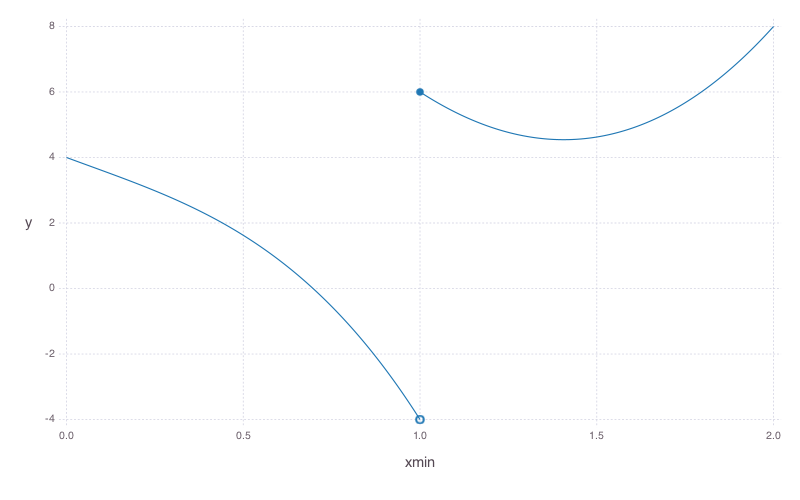
\includegraphics[width=\textwidth]{figures/allowed.png}
%         \caption{Admissible piecewise continuous function.}
%         \label{fig:allowed}
%     \end{subfigure}
%     \begin{subfigure}[t]{0.5\textwidth}\centering
%         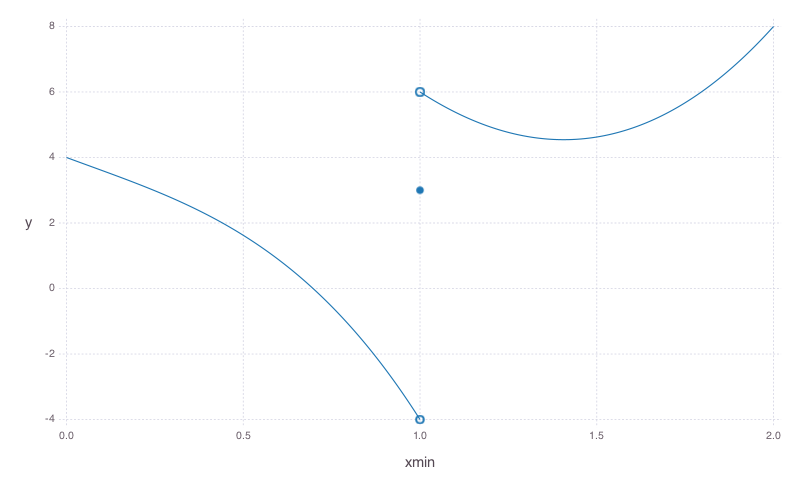
\includegraphics[width=\textwidth]{figures/not-allowed.png}
% 	    \caption{Not allowed!}
% 	    \label{fig:not-allowed}
%     \end{subfigure}
%     \caption{Examples to Definition \ref{definition-piecewise-continuous}.}
% \end{figure*}


\subsection{Definition DDE} \label{sec:definition-dde}

\begin{definition}[Delay Differential Equation]
    \label{definition-dde}

    Let $f:\R^n\times\R^n\rightarrow\R^n$ and $\tau > 0$.
    A functional equation of the form
    \begin{equation}
        x'(t) = f\left(x(t),x(t-\tau)\right)
    \end{equation}
    is called \textbf{Delay Differential Equation (DDE)} with \emph{constant, discrete delay}. It is \emph{autonomous}, since its right hand side $f$ is time independent.

    If the right hand side only depends on $x(t-\tau)$ and not on $x(t)$, we call the DDE \emph{pure}.

    A DDE can be equipped with an \textbf{initial condition}. It specifies the values of $x$ on $[-\tau, 0]$ on which the right hand side depends.

\end{definition}

Since we only consider autonomous DDEs, we can without loss of generality restrict to the case of initial time $t_0=0$.

The definition of a DDE can be extended to multiple constant discrete delays. For simplicity, we restrict here to a single delay.

\subsection{Definition of Solution} \label{sec:definition-of-solution}

\begin{definition}[Solution of DDE]
    \label{definition-solution-dde}

    A piecewise continuous function $x\in C^0_\text{pw}([-\tau,T],\R^n)$ is called \textbf{local solution} of the DDE (eq ??), if and only if there exists a $T>0$ such that $x|_{(0,T)}\in C^1((0,T),\R^n)$ with
    \begin{equation}
        x'(t) = f\left(x(t),x(t-\tau)\right)
    \end{equation}
    for all $t\in (0,T)$ and in $t=0$, it holds for the right-hand derivative \begin{equation}
        \lim_{h\searrow 0}\frac{x(h)-x(0)}{h}=f(x(0),x(-\tau))
    \end{equation}
    and obeys the initial condition:
    \begin{equation}
        x(t) = x_0(t) \quad\text{for } t\in [-\tau,0]
    \end{equation}
    on $[-\tau,0]$.

%TODO: differentiable in right rand point? need not derivative in right hand point

%TODO: Fortsetzbarkeit For example initial condition has jump, this point is limit for local solution.

    If the function $x$ is solution for all $T\in\R_{>0}$, it is called \textbf{global}.

\end{definition}

%TODO:
The notion of solution for an autonomous DDE as given above can be lifted to be a trajectory in the statespace
\begin{equation}
    \gamma_x:[0,T]\rightarrow\statespace,\\ t\mapsto\xbartaut{t}
\end{equation}

The \textbf{state} at time $t$ is a function which provides a time limited history up to the current time. This is all information needed to determine (using the DDE) to determine the solution for time $\geq t$. It is defined as $\xbartaut{t}(s)\defeq x(t+s)$ for $s\in [-\tau,0]$. In the case of $t=0$, we simplify the notation to $\xbartau \defeq \xbartaut{0}$.

This notion of solution is a \emph{dynamical systems} point of view which later turns out to be useful.

% \begin{figure}[h]\centering
%     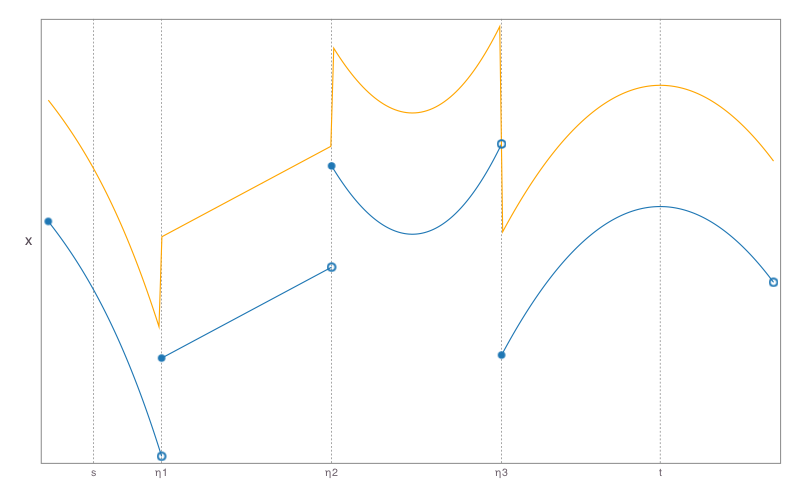
\includegraphics[width=\textwidth]{figures/multiple.png}
% 	\caption{Illustration of proof to Lemma \ref{lemma-continuity}}
% 	\label{fig:not-allowed}
% \end{figure}

% FIXME: This lemma is wrong. Show instead integrability of f(t,x_t)
\begin{lemma}
    \label{lemma-continuity}

    % Let $x:[\sigma-\tau,\sigma+T] \rightarrow \R^n$ be piecewise continuous (as in Definition \ref{definition-piecewise-continuous}) with the subdivision $\{t_0,\ldots,t_k\}$, i.e. there are $k$ subintervals.
    %
    % Then $t \mapsto x_t = x(t+\theta)$, where $\theta\in[-\tau,0]$, is a piecewise continuous mapping from $[\sigma,\sigma+T]$ into $\statespace$.
\end{lemma}

\begin{proof}
    % $x$ is piecewise continuous and hence uniformly piecewise continuous on the compact interval $I=[\sigma-\tau,\sigma+T]$.
    % i.e. uniformely continuous on each subinterval with stetiger Fortsetzung in right side.
    % \begin{equation}
    %     \forall\epsilon >0 \exists\delta_i >0 \forall t,s\in I_i: \quad \abs{t-s}<\delta_i \Rightarrow \norm{x(t)-x(s)}<\epsilon
    % \end{equation}
    % Let $\epsilon > 0$. $x|_{[t_i,t_{i+1}]}$ (with stetiger fortsetzung in right interval limit) is uniformly continuous, i.e. there is a $\delta_i > 0$ (for the given $\epsilon$), such that $\forall\,t, s \in [t_i,t_{i+1}]$ holds
    % % TODO: can use \leq ?
    % \begin{equation}
    %     \abs{t-s} < \delta_i \Rightarrow \norm{x(t)-x(s)} < \epsilon
    % \end{equation}
    %
    % Among the given $\delta_i$, choose the smallest as $\delta = \min_i \delta_i$.
    %
    % For any $i$ and $s,t\in [t_i,t_{i+1})\subset [\sigma,\sigma+T]$ with $\abs{t-s}<\delta$, it holds
    % \begin{equation}
    %     \supnorm{x_t - x_s} = \sup_{\theta\in [-\tau,0]}\norm{x(t+\theta) - x(s+\theta)} < \epsilon
    % \end{equation}
    % since $t+\theta, s+\theta \in I$
    % Hence $t \mapsto x_t$ is uniformely continuous on $[t_i,t_{i+1})$.
\end{proof}

\begin{definition}
    \label{definition-lipschitz}

    A function $f:\deff\rightarrow\R^n$ is called \textbf{locally Lipschitz continuous} in its second argument if and only if $\forall a,b\in\R,\forall M>0 \exists L>0$:
    \begin{equation}
        \norm{f(t,x,y) - f(t,\bar{x},y} \leq L\norm{x - \bar{x}}
    \end{equation}
    for all $t\in [a,b]$ and $\norm{x},\norm{\bar{x}},\norm{y}\leq M$.
\end{definition}

\begin{lemma}
    \label{lemma-bounded-f}

    Let $f:\deff\rightarrow\R^n$ be continuous and Lipschitz in its second argument.

    For any given compact interval $[a,b]$ ans $M>0$ there exists a bound $K>0$
    \begin{equation}
        \norm{f(t,x,y)}\leq K
    \end{equation}
    where $t\in[a,b]$ and $\norm{x},\norm{y}\leq M$.
\end{lemma}

\begin{proof}
    Let $L$ be the Lipschitz constant of $f$ for given $[a,b]$ and $M$. Then
    \begin{multline}
        \norm{f(t,x,y)} \leq \norm{f(t,x,y) - f(t,0,y)} + \norm{f(t,0,y)}\\
        \leq L\norm{x-0} + \norm{f(t,0,y)} \leq LM+P = K
    \end{multline}
    when $t\in[a,b]$ and $\norm{x},\norm{y}\leq M$. We used the continuity of $f$ for the existence of
    \begin{equation}
        P = \max_{s\in [a,b],y}\norm{f(s,0,y)}
    \end{equation}
\end{proof}

\begin{lemma}
    \label{lemma-integral-equation}

%TODO: solving dde equiv to solving integral equation??? (-\textgreater{} Lemma) and compare with ODE lecture notes

    Finding a solution of the DDE (??) is equivalent to solving the integral equation

    \begin{equation}
        x(t) = x_0(0) + \int_0^t g(\bar{x}_{\tau,s})ds
    \end{equation}
    and is continuous in t.
\end{lemma}

\begin{proof}
integrate from discontinuity of $\xbartaut{t}$ to discontinuity and proof stetige fortsetzbarkeit at these points
\end{proof}

\subsection{Method of Steps} \label{sec:method-of-steps}
for $t\in [0,\tau]$, $x$ must satisfy the following ordinary initial value problem obtained by plugging the initial function into equation (??). For suitable $f$ and $x_0$, the existence (and uniqueness) of a solution on $[0,\tau]$ is guaranteed by ODE theory (\ldots{} or Picard-Lindelöf theorems).

This procedure can then be applied repeatedly to extend the obtained solution by steps of length $\tau$.

\subsection{Existence and Uniqueness of Solutions} \label{existence-and-uniqueness-of-solutions}

$f$ Lipschitz with piecewise continuous initial function have existence and uniqueness ???? smoothing

\begin{theorem}
    \label{theorem-solution-existence}
    Consider the Delay Differential Equation

%TODO: do we need global existence or just local?

%TODO: this DDE is more general than in definition above

    \begin{equation}
        \begin{cases}
            x' = f(t,x(t),x(t-\tau)) & \text{for } t\geq\sigma\\
            x(t) = x_\sigma(t-\sigma)     & \text{for } t\in [\sigma-\tau,\sigma]
        \end{cases}
    \end{equation}

    with $f:\deff\rightarrow\R^n$ continuous and satisfying the (local) Lipschitz condition (\ref{definition-lipschitz}).
    % \begin{equation}
    %     \forall M>0\,\exists L>0\,\forall x,y\in C^0([-\tau,0],\R^n) : \supnorm{x},\supnorm{y}\leq M\Rightarrow\norm{f(x)-f(y)} \leq L\supnorm{x-y}
    % \end{equation}
    % where $\norm{\cdot}$ denotes the Euclidian norm on $\R^n$ and $\supnorm{\cdot}$ the supremum norm of the Banach space of continuous functions on $[-\tau,0]$.

    Then for each \textbf{initial condition} $x_\sigma\in\statespace$ and start time $\sigma$, there \textbf{exists} a \textbf{unique local solution} of the DDE on a time interval $[\sigma-\tau, \sigma+T]$. $T>0$ depends on in the initial condition, in terms of its bound and discontinuity points.
\end{theorem}
The proof is smiliar to the proof of ... given in \cite{smith2010introDDE}.
\begin{proof}
    The initial condition is bounded by $\supnorm{x_\sigma}\leq M$.
    Let $K>0$ be the bound for $f$ from Lemma \ref{lemma-bounded-f} on the set $[\sigma,\sigma+t_1] \times \{x\in R^n: \norm{x}\leq 2M\}\times \{y\in R^n: \norm{y}\leq M\}$ and $L>0$ the Lipschitz constant for that set. Choose $T=\min\{t_1-\tau ?, \frac{M}{K}\}$

    We construct a series which approximates the solution.
    Set
    \begin{equation}
        x^{(0)}(t)= \begin{cases}
            x_\sigma(0) & t\in [\sigma,\sigma+T]\\
            x_\sigma(t-\sigma) & t\in [\sigma-\tau,\sigma]
        \end{cases}
    \end{equation}
    For $m\in\N_0$ define
    \begin{equation}
        x^{(m+1)}(t)= \begin{cases}
            x_\sigma(0) + \int_\sigma^t f(s,x^{(m)}(s),x^{(m)}(s-\tau))\dx{s} & t\in [\sigma,\sigma+T]\\
            x_\sigma(t-\sigma) & t\in [\sigma-\tau,\sigma]
        \end{cases}
    \end{equation}
    It holds for all m $\forall\,t\in [\sigma-\tau,\sigma]$
    \begin{equation}
        \norm{x^{(m+1)}(t)-x^{(m)}(t)}=0
    \end{equation}
    We show by induction that
    \begin{equation}
        \norm{x^{(m)}(t)-x^{(m-1)}(t)} \leq \frac{K}{L}\frac{L^m (t-\sigma)^m}{m!}
    \end{equation}
    $\forall\,t\in [\sigma,\sigma+T]$.
    The IA holds, since obviously $\norm{x^{(0)}(t)}\leq M$
    \begin{equation}
        \norm{x^{(1)}(t)-x^{(0)}(t)} = \norm{\int_\sigma^t f(s,x^{(0)}(s),x^{(0)}(s-\tau))\dx{s}} \leq K(t-\sigma)
    \end{equation}
    Since for any $m$, it holds
    \begin{equation}
        \norm{x^{(m)}}\leq \norm{x_\sigma(0)} + \int_\sigma^t \norm{f(s,x^{(m)}(s),x^{(m)}(s-\tau))}\dx{s}
        \leq M + K(t-\sigma) \leq M+KT \leq 2M
    \end{equation}
    we can apply Lipschitz in the induction step
    \begin{align}
        \norm{x^{(m+1)}(t)-x^{(m)}(t)} &= \norm{\int_\sigma^t f(s,x^{(m)}(s),x^{(m)}(s-\tau)) - f(s,x^{(m-1)}(s),x^{(m-1)}(s-\tau))\dx{s}}\\
        & \leq K \int_\sigma^t \norm{x^{(m)}(s) - x^{(m-1)}(s)}\dx{s} \leq \frac{L^m K}{m!} \int_\sigma^t (s-\sigma)^m\dx{s}\\
        & = \frac{L^m K}{(m+1)!}(t-\sigma)^{m+1}
    \end{align}
    We use this bound and the triangle inequality in
    \begin{equation}
        \norm{x^{(t)}(t)-x^{(k)}(t)}\leq \norm{x^{(m)}(t)-x^{(m-1)}(t)} + \norm{x^{(m-1)}(t)-x^{(m-2)}(t)} +\ldots + \norm{x^{(k+1)}(t)-x^{(k)}(t)}\\
        \leq \frac{K}{L}\frac{L^m (t-\sigma)^m}{m!} + \frac{K}{L}\frac{L^{m-1} (t-\sigma)^{m-1}}{(m-1)!} +\ldots +\frac{K}{L}\frac{L^{k+1} (t-\sigma)^{k+1}}{(k+1)!}\\
        \leq \frac{K}{L}\sum_{i=k+1}^\infty \frac{(LT)^i}{i!}
    \end{equation}
    for any $k\in\N$ and $m\geq k$ and $t\in [\sigma,\sigma+T]$.
    This is the tail of the convergent exponential series and hence it converges to zero for $k\rightarrow\infty$.
    Since $x^{(m)}$ is continuous on $[\sigma,\sigma+T]$, this Cauchy sequence admits a limit $x$ in the Banach space $C^0([\sigma,\sigma+T],\R^n)$. Extend again to $[\sigma-\tau,\sigma]$ with $x_\sigma$, so $x\in C^0_\text{pw}([\sigma-\tau,\sigma],\R^n)$.


    Due to the uniform convergence of $x^(m)\rightarrow x$, we get uniform convergence of
    \begin{equation}
        f(s,x^{(m)}(s),x^{(m)}(s-\tau)) \rightarrow^{m\rightarrow\infty} f(s,x(s),x(s-\tau))
    \end{equation}
    and hence the integral and the limit process swap and by
    \begin{equation}
        x(t) = \lim_{m\rightarrow\infty} x^{(m+1)} = x_\sigma(0) + \lim_{m\rightarrow\infty}\int_\sigma^t f(s,x^{(m)}(s),x^{(m)}(s-\tau))\dx{s} = \int_\sigma^t f(s,x(s),x(s-\tau))\dx{s}
    \end{equation}
    it follows that $x$ solves the integral equation.
    This proofs the existence of a solution to the DDE. It remains to show uniqueness.

    % TODO: can one solution be on [\sigma, T_2] with T_2<T ?
    Let $x$ and $\bar{x}$ be two solutions of the DDE on $[\sigma,\sigma+T]$.
    By Lemma \ref{lemma-integral-equation} they are equivalent to solutions of the integral equations
    \begin{equation}
        x(t) = x_\sigma + \int_\sigma^t f(s,x(s,\xtau{s}))\dx{s}
    \end{equation}
    and
    \begin{equation}
        \bar{x}(t) = x_\sigma + \int_\sigma^t f(s,\bar{x}(s,x_0{\sigma-s}))\dx{s}
    \end{equation}

    For $t\in [\sigma,T]$, we set
    \begin{align*}
        \rho(t) &= \norm{x(t)-\bar{x}(t)} \leq \int_\sigma^t \norm{f()-f()}\dx{s}\\
        & \leq L \int_\sigma^t \norm{x(s)-\bar{x}(s)}\dx{s} = L \int_\sigma^t \rho(s)\dx(s)\\
        & L \int_\sigma^t \e{-\alpha s}\rho(s)\e{\alpha s}\dx{s} \leq L \sup_{s\in [\sigma,T]}(\e{-\alpha s}\rho(s))\int_\sigma^t \e{\alpha s}\dx{s}\\
        & \leq\frac{L}{\alpha}\e{\alpha s} \sup_{s\in [\sigma,T]}(\e{-\alpha s}\rho(s))
    \end{align*}
    Choosing $\alpha=2L$ and multiplying with $\e{-\alpha t}>0$ leads to
    \begin{equation}
        \rho(t)\e{-2Lt} \leq \frac{1}{2}\sup_{s\in [\sigma,T]}(\e{-\alpha s}\rho(s))
    \end{equation}
    for all $t\in [\sigma,T]$
    \begin{equation}
        0 \leq sup_{t\in [\sigma,T]}(\rho(t)\e{-2Lt}) \leq \frac{1}{2}\sup_{s\in [\sigma,T]}(\e{-\alpha s}\rho(s))
    \end{equation}
    and hence $\rho(t)=0$ for all $t\in [\sigma,T]$, which means $x(t)=\bar{x}(t)$.

    % TODO: still needed?
    just proof existence/uniqueness on each peace of continuity proof continuity at knots with Lemma of integral equ

\end{proof}

\begin{corollary}
    \label{cor:continuability-of-solution}
    If in Theorem \ref{theorem-solution-existence} $T=t_1-\tau$, can reapplay theorem with starting point $\sigma=\sigma_{old}+t_1-\tau$. Get existence of unique solution on $[\sigma-\tau,\sigma+S]$ with $S>T$.
\end{corollary}

\begin{corollary}
    \label{corollary}
    If f is polynomial in $t$, $x(t)$ and $x(t-\tau)$ then theorem holds

    polynomial -> continuously differentiable -> locally Lipschitz
% IDEA: can show? init cond bounded by M, and loc sol bounded by M, get glob sol since f glob Lip on set of bounded inputs?

%TODO: can write DDE (eq??) from definition as

\begin{equation}
    \begin{cases}
        x'=f(\xbartaut{t})\defeq g(\xbartaut{t}(0),\xbartaut{t}(-\tau)) &\text{for } t\geq 0\\
        x(t)=x_0(t) & \text{for } t\in[-\tau,0]
    \end{cases}
\end{equation}
\end{corollary}

\begin{proof}

\end{proof}

% TODO: non-autonomous -> autonomous

\subsection{Example}\label{example}
The basic ODE IVP
\begin{equation}
    \begin{cases}
        x'(t) = -x(t)\\
        x(0) = x_0
    \end{cases}
\end{equation}
has the solution $x(t)=x_0 e^{-t}$. However the similiar DDE
\begin{equation}
    \begin{cases}
        x'(t) = -x(t-\tau) & t\geq 0\\
        x(t) = x_0(t) & -\tau\leq t\leq 0
    \end{cases}
\end{equation}
has a much richer dynamics, but solution (as series) for $x_0\equiv 1$, can compute first solutions by method of steps. \ldots{}

\begin{figure}[h]\centering
    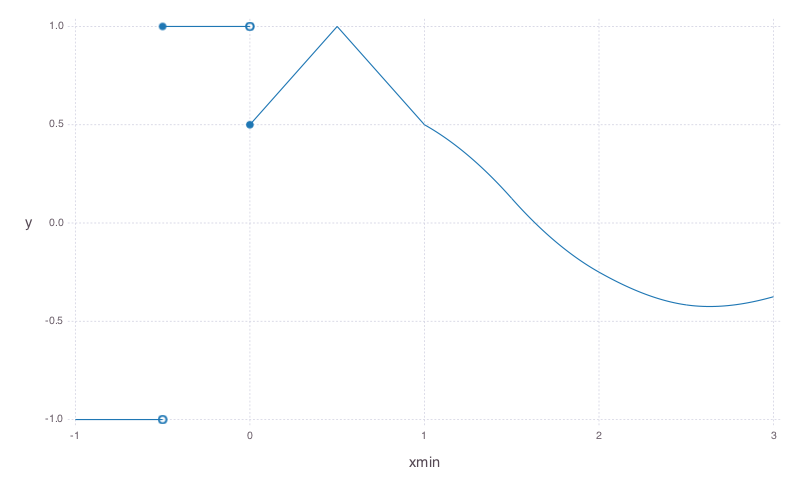
\includegraphics[width=\textwidth]{figures/piecewise-initial-function.png}
	%\caption{}
	\label{fig:not-allowed}
\end{figure}

\subsection{Definition}\label{definition}

\section{Hybrid Programs with DDEs}\label{hybrid-programs-with-ddes}

    We extent classic hybrid programs (\HP) and \dL formulae with syntax, semantics, axiomatization and proof rules for DDEs.
    %Is a super set, \dL is a fragment

    \subsection{Example}
        \label{example-hp-cars}
        To motivate the need of being able to treat Delayed Differential Equations in hybrid programs, we present some examples.

        \subsubsection{Leading and Following Car}

        \subsubsection{Network Induced Delay in Control Loops}

    \subsection{Syntax}
        \label{sec:syntax}

        \paragraph{Terms}
            \label{sec:terms}

            We extent the grammar defining \textbf{terms} with a symbol for a \textbf{delayed variable}
            % FIXME: replace ::=
            % FIXME: replace |
            % FIXME: replace x'
            \begin{equation}
                \theta,\eta ::= x|\xtau|x'|c|\theta+\eta|\theta\cdot\eta
            \end{equation}

    The grammars for hybrid programs and \dL formulas remain unchanged.


    \subsection{Semantics}
        \label{sec:semantics}
        \begin{equation}
            \imodels[\I]{\phi}{x}
        \end{equation}

        Following the remark to the solution of a DDE, we augment the \textbf{state space} in \dL to $\statespace$, the set of piecewise continuous functions on $[-\tau,0]$, as defined in \ref{definition-piecewise-continuous}.

        %TODO: need $\xbartau$

        We senote by $\states$ the set of states. A state $\omega\in\states$ is a mapping
        \begin{equation}
            \omega : \mathcal{V}\cup\mathcal{V'}\rightarrow\statespace
        \end{equation}
        that assigns a \emph{history} (function) $\xbartau$ to each variable symbol and

        %FIXME: need diff var symbol? can determine derivative from x? need pw diffable?

        % TODO: Abgrenzung zu Trace Semantics
        % The temporal character of delay differential equations (they depend on their own temporal evolution with limited horizon) suggests the introduction of trace semantics.
        %
        % However, we go the way of introducing transition semantics with an augmented state space.

        \subsubsection{Terms}
            \label{sec:terms-semantic}

            The semantic of the new symbol $\xtau$ depends on the context in which the term occures:
            \begin{itemize}
                \item in a hybrid program: $\imodel{\I}{\xtau} = \imodel[\nu]{}{x(t-\tau)} = \nu(x)(-\tau)$
                \item in a formula: \begin{equation}
                    % FIXME: rechte seite noch nicht korrekt
                    \imodel[]{}{\phi(\xtau)} =
                    \{\nu\in\states : \lforall{t\in[-\tau,0]}{\phi(\nu(x)(t))} \}
                \end{equation}
            \end{itemize}

            The semantics of the variable symbols in terms are given by
            \begin{equation}
                \imodel[\nu]{}{x}=\nu(x)(0)
            \end{equation}
            and
            \begin{equation}
                \imodel[\nu]{}{x'}=\nu(x')(0)
            \end{equation}
            In the precondition, no values are associated to the differential symbols. In general, the initial function is only piecewise continuous.
            Since for later time instances, the values of the differential symbols derive from the DDE, they become (locally) smooth function.


            When we write $x$ we mean $x(t)$.

        \subsubsection{\dL semantics}
            With the semantics of terms if follows for the meaning of $\dbox{\alpha}{\phi}$, that $\phi$ must only hold up to time $\tau$ before leaving the \HP $\alpha$. It is possible, that $\phi$ was not verified before, while \textit{executing} the \HP.

            However when we apply the Rule of steps, we get the validity of $\phi$ for the entire trace.

        \subsubsection{Hybrid Programs}
            \label{sec:hp-semantics}

            The transition semantic of a hybrid program $\alpha$ is inductively given by a binary reachability relation $\rho(\alpha)\subseteq\states\times\states$. Since the state space has been replaced, we need to redefine the semantics:

            The \emph{discrete assignment} does not rewrite history, but changes only the value at the current time instant:
            \begin{equation}
            \rho(x:=\theta) = \left\{(\nu,\omega): \omega = \nu \text{ except } \omega(x)=\left(t\mapsto\begin{cases}\imodel{\I}{\theta} & t=0\\ \nu(t) &t\in[-\tau,0)\end{cases}\right)\qquad\right\}_.
            \end{equation}
            This assignment is the actual reason why we need to consider piecewise continuous evolutions.

            %TODO: super dense time: multiple assignments

            Using the extended syntax, we can write down both a delay differential equation and an ordinary differential equation in the form $x'=\theta$, where $\theta=f(x,\xtau)$ with a polynomial $f$.
            \begin{equation}
                \rho(x'=\theta\,\&\,\chi) = \left\{
                    (\varphi(0),\varphi(s))\,:\,\varphi(t)\models x'=\theta\,\wedge\,\varphi(t)(0)\models\chi\,\forall\,0\leq t\leq s\text{ for a solution } \varphi:[0,s]\rightarrow\states \right\}
            \end{equation}
            As a solution, $\varphi$ needs to fulfill
            \begin{equation}
                \varphi(t)(x')(0) \defeq \DD{\varphi(\zeta)(x)(0)}{\zeta}(t) \stackrel{!}{=} \imodel[]{\varphi(t)}{\theta}
            \end{equation}
            Remember that a $\xtau$ mentioned in $\theta$ here means $\varphi(t)(x)(-\tau)$.
            And so needs $\chi$ always just hold at the current time instant (and not over the entire interval $[-\tau,0]$). The same case for $\ptest\psi$.

            % TODO: what about [a;b]p. is [a][b]p correct?

\section{Delay Differential Dynamic Logic}
    \label{sec:delay-differential-dynamic-logic}

    \subsection{Proof Rules}
        \label{sec:seq-calc-proof-rules}

        We keep the standard sequent calculus proof rules

        \begin{calculus}
          \cinferenceRule[andR|$\land$R]{and right proof rule}
           {
           \linferenceRule[sequent]
           {\lsequent{\Gamma} {p,\Delta}
           &\lsequent{\Gamma} {q,\Delta}
           }
           {\lsequent{\Gamma} {p\land q,\Delta}}
           }{}
          \cinferenceRule[andL|$\land$L]{and left proof rule}
           {
           \linferenceRule[sequent]
           {\lsequent{\Gamma, p, q} {\Delta}}
           {\lsequent{\Gamma, p\land q} {\Delta}}
           \quad
           }{\text{no side condition}}
          \cinferenceRule[implyR|$\limply$R]{imply right proof rule}
           {
           \linferenceRule[sequent]
           {\lsequent{\Gamma,p} {q,\Delta}}
           {\lsequent{\Gamma} {p\limply q,\Delta}}
           }{}
        \end{calculus}


    \subsection{Dynamic Axioms}
        \label{sec:dynamic-axioms}

% TODO: History Axiom
        \subsubsection{History Axiom}
            \label{history-axiom}
            Just replace symbol by its semantical meaning
            The occurence of $\xbartau$ in expressions can be replaced by turning the (implicitely existing) time variable explicit, i.e.\
            \begin{equation}
                F(\xbartau) \leftrightarrow \forall\,-\tau\leq t\leq 0\, F(x(t))
            \end{equation}

        \subsubsection{Axiom of Steps}
            \label{sec:axiom-of-steps}
            The \emph{Method of Steps} presented above translates into an axiom.
            %It allows to partially unwind an autonomous DDE given a analytic representation of its solution.

            % Let $\theta_0$ and $\theta$
            \begin{equation}
                % \xbartau = \theta_0 \rightarrow [x'=\theta(\xbartaut{t})]\phi
                % \leftrightarrow
                % \left(\forall 0\leq t\leq\tau: [x:= y(t)]\phi \right)
                % \wedge \xbartaut{\tau} = y \rightarrow [x'=\theta (\xbartaut{t})]\phi
                \dbox[]{\hevolvein{x'=\rho(x,\xtau)}{\chi}}{\phi}
                \lbisubjunct
                \dbox[]{\prepeat{(\hupdate{\humod{t}{0}};\hevolvein{t'=1\syssep x'=\rho(x,\xtau)}{(\chi\land 0\leq t\leq\tau)})}}{\phi}
            \end{equation}
            % where $\forall 0\leq t\leq\tau$, $y'(t)=\theta(\theta_0)$, i.e.\ $y$ is a local solution of the DDE. The solution must be expressible in polynomial form so that the axiom leads to decidable arithmetic.

            (Since the DDE is autonomous, we can emit the time index.)

            \begin{proof}
                apply methods of steps
            \end{proof}

    \subsection{Proof Rules}
        \label{sec:proof-rules}

        \begin{calculus}
            % TODO: [;]
            %\cinferenceRule[[;]|]{}{\linferenceRule[]{}{}}{}
            % TODO: replace := by command
            \cinferenceRule[assignb|$\mathrel{{:}{=}}$]{discrete assignment}{
                \linferenceRule[sequent]{
                    \lsequent{\Gamma,x=e}{P,\Delta}
                }{\lsequent{\Gamma}{\dbox{\hupdate{\humod{x}{e}}}{P},\Delta}}
            }{if $x\notin\Gamma,\Delta$}
            \cinferenceRule[loop|loop]{loop invariant}{
                \linferenceRule[sequent]{
                    \lsequent{\Gamma}{J,\Delta}
                    &\lsequent{J}{\dbox{\alpha}{J}}
                    &\lsequent{J}{P}
                }{\lsequent{\Gamma}{\dbox{\prepeat{\alpha}}{P},\Delta}}
            }{}
            \cinferenceRule[DC|DC]{differential cut}{
                \linferenceRule[sequent]{
                    \lsequent{\Gamma}{\dbox{\hevolvein{x'=f(x)}{\chi}}{r(x)},\Delta}
                    &\lsequent{\Gamma}{\dbox{\hevolvein{x'=f(x)}{\chi\land r(x)}}{P}}
                }{\lsequent{\Gamma}{\dbox{\hevolvein{x'=f(x)}{\chi}}{P},\Delta}}
            }{}
            \cinferenceRule[dI|dI]{differential invariant}{
                \linferenceRule[sequent]{
                    \lsequent{\Gamma,Q}{P,\Delta}
                    % FIXME: replace ':= by correct command
                    &\lsequent{Q}{\dbox{x':=f(x)}{(P)'}}
                }{\lsequent{\Gamma}{\dbox{\hevolvein{x'=f(x)}{\chi}}{P},\Delta}}
            }{}
            \cinferenceRule[dW|dW]{differential weakening}{
                \linferenceRule[sequent]{
                    \lsequent{\Gamma}{\lforall{x}{(\chi\limply P)},\Delta}
                }{\lsequent{\Gamma}{\dbox{\hevolvein{x'=f(x)}{\chi}}{P},\Delta}}
            }{}
        \end{calculus}

        % TODO: Rule of Steps
        \subsubsection{Rule of Steps}
            \label{sec:rule-of-steps}

            condition valid for initial condition and given condition for a $s\leq t$ then condition holds after dde-evolution of max time tau and safety follows from condition then condition holds after dde with mentioned initial condition
            \begin{equation}
            \frac{\Gamma(\xbartaut{0})\rightarrow F(\xbartaut{0})\quad F(\xbartaut{s})\rightarrow [x'=\theta(\xbartaut{t})\,\&\,t\leq\tau]F(\xbartaut{t}) \quad F(\xbartaut{t})\rightarrow\phi}{\Gamma(\xbartaut{0}) \rightarrow [x'=\theta(\xbartaut{t})]\phi}
            \end{equation}

            \begin{calculus}
                % FIXME: \landS -> steps
                \cinferenceRule[steps|steps]{steps proof rule}{
                    \linferenceRule[sequent]{
                        \lsequent{\Gamma}{F,\Delta}
                        &\lsequent{t=0,F(\theta(t-\tau))}{\dbox[]{\hevolvein{t'=1\syssep x'=\rho(x,\theta(t-\tau))}{(\chi\land 0\leq t\leq\tau)}}{F}}
                        &\lsequent{F}{\phi}
                    }{
                        \lsequent{\Gamma}{\dbox[]{\hevolvein{x'=\rho(x,\xtau)}{\chi}}{\phi},\Delta}
                    }
                }{}
            \end{calculus}

        \subsubsection{Delay Differential Induction}
            \label{sec:delay-differential-induction}

            \begin{sequentdeduction}
                \linfer[]{
                    \lsequent{\Gamma}{F,\Delta}
                    &\lsequent{\chi,0\leq t\leq\tau,F(\theta(t-\tau))}{\dbox[]{\hevolve{x':=\rho(x,\theta(t-\tau))}}{(F)'}}
                    &\lsequent{F}{\phi}
                }{
                    \lsequent{\Gamma}{\dbox[]{\hevolvein{x'=\rho(x,\xtau)}{\chi}}{\phi,\Delta}}
                }
            \end{sequentdeduction}

            %\begin{proof}\small
            \begin{sidewaysfigure}\footnotesize
            \centering
            \begin{sequentdeduction}[]
                \linfer[Axsteps]{
                    \linfer[loop]{
                        % FIXME: formel zu hoch
                        \lsequent{\Gamma(\xtau)}{F(\xtau),\Delta}
                        &\linfer[assignb,seq]{
                            \linfer[DC]{
                                \linfer[dI]{
                                    \linfer[Hist]{
                                        \linfer[id]{
                                            \lclose
                                        }{
                                            \lsequent{\lforall{s\in[-\tau,0]}{F(\theta(s))}}{\lforall{r\in[-\tau,0]}{F(\theta(r))}}
                                        }
                                    }{
                                        \lsequent{F(\xtau),t=0,\chi, 0\leq t\leq\tau, F(x(t-\tau))}{F(\xtau)}
                                    }
                                    &\linfer[]{
                                        \lsequent{}{}
                                    }{
                                        \lsequent{\chi, 0\leq t\leq\tau, F(x(t-\tau)))}{\dbox{t':=1, x':=\rho(x,\xtau)}{(F)'}}
                                    }
                                }{
                                    \lsequent{F,t=0}{\dbox{\hevolvein{t'=1\syssep x'=\rho(x,\xtau)}{(\chi\land 0\leq t\leq\tau\land F(x(t-\tau)))}}{F}}
                                }&\linfer[]{
                                    \linfer[dW]{
                                        \linfer[allR]{
                                            \linfer[implR]{
                                                \linfer[]{
                                                    \lclose
                                                }{
                                                    \lsequent{\lforall{s\in[-\tau,0]}{F(\theta(s))},t=0,\chi(r,y),0\leq r\leq\tau}{F(\theta(r-\tau))}
                                                }
                                            }{
                                                \lsequent{\lforall{s\in[-\tau,0]}{F(\theta(s))},t=0}{\chi(r,y)\land 0\leq r\leq\tau\limply F(\theta(r-\tau))}
                                            }
                                        }{
                                            \lsequent{\lforall{s\in[-\tau,0]}{F(\theta(s))},t=0}{\lforall{(t,x)}{(\chi\land 0\leq t\leq\tau\limply F(\theta(t-\tau)))}}
                                        }
                                    }{
                                        \lsequent{\lforall{s\in[-\tau,0]}{F(\theta(s))},t=0}{\dbox{\hevolvein{t'=1\syssep x'=\rho(x,\theta(t-\tau))}{(\chi\land 0\leq t\leq\tau)}}{F(\theta(t-\tau))}}
                                    }
                                }{
                                    \lsequent{F(\xtau),t=0}{\dbox{\hevolvein{t'=1\syssep x'=\rho(x,\xtau)}{(\chi\land 0\leq t\leq\tau)}}{F(x(t-\tau))}}
                                }
                            }{
                                \lsequent{F,t=0}{\dbox[]{\hevolvein{t'=1\syssep x'=\rho(x,\xtau)}{(\chi\land 0\leq t\leq\tau)}}{F}}
                            }
                        }{
                            \lsequent{F(\xtau)}{\dbox[]{\hupdate{\humod{t}{0}}; \hevolvein{t'=1\syssep x'=\rho(x,\xtau)}{(\chi\land 0\leq t\leq\tau)}}{F}}
                        }
                        \lsequent{F(\xtau)}{\phi}
                    }{
                    \lsequent{\Gamma(\xtau)}{\dbox{\prepeat{(\hupdate{\humod{t}{0}}; \hevolvein{t'=1\syssep x'=\rho(x,\xtau)}{(\chi\land 0\leq t\leq\tau))}}}{\phi,\Delta}}}
                }
                {\lsequent{\Gamma(\xtau)}{\dbox{\hevolvein{x'=\rho(x,\xtau)}{\chi}}{\phi,\Delta}}}
            \end{sequentdeduction}
            \end{sidewaysfigure}
            \normalsize
            %\end{proof}

        \subsubsection{Delay Differential Invariant}
            \label{sec:elay-differential-invariant}

            Mentioning $\xtau$ in the invariant differential invariant is not permitted, since derivation would lead to the occurrence of the symbol $x_{2\tau}$, whose properties are out of the scope of the current state.

            %TODO: much doubt if that is sound
            \begin{equation}
                \frac{H\wedge\forall\,t-\tau\leq s<t: F(x(s))\rightarrow (F')^{\theta}_{x'}}{F(\xbartau)\rightarrow [x'=\theta(\xbartaut{t})\,\&\,(H\wedge t\leq\tau)]F(\xbartaut{t})}
            \end{equation}

% TODO: Example
        \subsubsection{Example}
            \label{sec:example}
            We want to proof the safety condition $\phi\equiv(-1\leq x\wedge x\leq 1)$ for the continuous program with delay differential equation
            \begin{equation}
                \forall\,t\in[-\tau,0]:\,-1\leq\xbartaut{0}(t)\wedge\xbartaut{0}(t)\leq 1
                \rightarrow
                [x'=-\xtau] (\forall\,s\in[-\tau,0]:\,-1\leq\xbartaut{t}(s)\wedge\xbartaut{t}(s)\leq 1)
            \end{equation}
            in explicit quantified representation. It can be simplified by using an implicit time variable and a context depending meaning of $\xtau$
            \begin{equation}
                -1\leq\xtau\leq 1 \rightarrow [x'=-\xtau]\phi.
            \end{equation}

            We apply the rule of steps using the safety condition $\phi$ as step condition $F(x)\equiv(\forall\,t\in[-\tau,0]:\,-1\leq x(t)\wedge x(t)\leq 1)$.

            The first and third premisses hold. The second by ??? (delay differential invariant)

            Use the algebraic differential invariant $F\equiv(-1\leq x^3\wedge x^3\leq1)$, which is valid for the initial condition. Differentiation leads to the inequalities, which needs to be shown $\forall t\in[0,\tau]$
            \begin{equation}
                0\leq 3\,x(t)^2 x'(t) = -3\,x(t)^2 \xtau(t)
            \end{equation}

            This holds since










\nocite{*}
\bibliographystyle{plain}
\bibliography{Bibliography}

\end{document}
